%% -*- coding: utf-8 -*-
\documentclass[12pt,a4paper]{report}
\usepackage[left=2cm,right=2cm,
    top=2cm,bottom=2cm,bindingoffset=0cm]{geometry} 
\usepackage[utf8]{inputenc}
\usepackage[english,russian]{babel}
\usepackage{indentfirst}
\usepackage{misccorr}
\usepackage{graphicx}
\usepackage{amsmath}
\usepackage{amsfonts}
\usepackage{amssymb}
\setcounter{page}{2}
\begin{document}

\begin{titlepage}
\newpage
  \begin{center}
     
    Санкт-Петербургский Политехнический Университет Петра Великого \\
    
    Институт компьютерных наук и технологий \\
    
    Кафедра компьютерных систем и программных технологий
    \end{center}
    
    \vspace{15em}
    \begin{center}
    \textsc{Лабораторная работа №2}\\
    \vspace{5mm}
    \textsc{Ряд Фурье. Преобразование Фурье.\\
           Корреляция}
    	
   \end{center}
\vspace{10em}

\newlength{\ML}
\settowidth{\ML}{«\underline{\hspace{0.7cm}}» \underline{\hspace{2cm}}}
\hfill\begin{minipage}{0.45\textwidth}
\vfill
  Руководитель \\
  \\
  \underline{\hspace{\ML}} Богач Н.\,В.\\
 
\end{minipage}%
\bigskip

\hfill\begin{minipage}{0.45\textwidth}
  Выполнил\\
  \\
  \underline{\hspace{\ML}} Солдатова Е.\,И.\\
  группа 33501/3
\end{minipage}%

\vspace{\fill}
\begin{center}
    
  Санкт-Петербург\\
   2018 
\end{center}
\end{titlepage}

\paragraph{1. Цель работы\\\\}
Получить представление о спектрах телекоммуникационных
сигналов.

\paragraph{2. Постановка задачи\\\\}
– Для сигналов, построенных в лабораторной работе №1, вы-
полните расчет преобразования Фурье. Перечислите свойства
преобразования Фурье.

– С помощью функции корреляции найдите позицию синхропосылки [101] в сигнале [0001010111000010]. Получите пакет
данных, если известно, что его длина составляет 8 бит без
учета синхропосылки. Вычислите корреляцию прямым методом, воспользуйтесь алгоритмом быстрой корреляции, сравните время работы обоих алгоритмов.

– Быстрая корреляция.

\paragraph{3. Теоретическая часть \\\\}
\textbf{Свойства преобразования Фурье\\}
Рассмотрим сигналы: $f (t)$ и $ g (t)$. Их спектральные функции: $F(\omega)$ и $G(\omega)$ соответственно.

• Cуммирование функций: линейная комбинация преобразованных равна результату преобразования линейных комбинаций.
  \begin{center}
Если $s(t) = \alpha f(t) + \beta g(t)$, то $S(\omega) = \alpha F (t) + \beta G(t)$.
  \end{center}
  
  • Свертывание функций: произведение спектров может сказать о том, как система воздействует на сигнал.
  \begin{center}
$h(x)=f \otimes g =\int_{-\infty}^{\infty} f(y)(x-y)dy$
  \end{center}
  
• Смещение функций: можно двигать сигнал по оси времени, это изменит его фазовый спектр на известную величину $\tau$.

• Изменение масштаба аргумента функций: спектр исходной функции изменяется в ширине обратно пропорционально сигналу.

• Дифференцирование функций.

• Интегрирование функций. 
\\

\textbf{Корреляция сигналов\\}
Корреляция применяется для измерения степени схожести двух сигналов. Взаимная корреляция:

\begin{figure}[h!]
\center{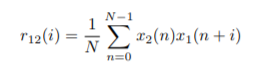
\includegraphics[width=0.4\linewidth]{1}}
\end{figure}
где n - временные отсчеты, i - задержка (число отсчетов, на которые сигнал x2 отстает от сигнала x1).

Для сигналов конечной длительности функция взаимной корреляции определяется следующим
образом:
\begin{figure}[h!]
\center{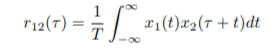
\includegraphics[width=0.35\linewidth]{2}}
\end{figure}
\newpage
Расчет корреляции можно ускорить, используя теорему о корреляции, которая формулируется так:

\begin{figure}[h!]
\center{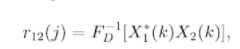
\includegraphics[width=0.35\linewidth]{Corr_exp}}
\end{figure}

Данный подход требует выполнения двух дискретных преобразований Фурье (ДПФ) и одного обратного ДПФ. Если число элементов в последовательностях x1(n) и x2(n) достаточно велико, то быстрой корреляцией
ответ будет получен быстрее, чем при расчете с помощью взаимной корреляции.

\paragraph{4. Ход работы \\\\}
Зададим синусоидальный и прямоугольный сигналы так же, как делали это в лабораторной работе 1. Затем посмотрим их спектры. 

Рассмотрим алгоритмы обычной корреляции (xcorr) и быстрой корреляции. Сравним время их выполнения.

Текст программы:\\
x = [ 0 0 0 1 0 1 0 1 1 1 0 0 0 0 1 0 ];\\
y = [ 1 0 1 ];\\
figure;\\
tic;\\
Corrcross = xcorr(x,y);\\
time = toc\\
subplot(2,1,1)\\
stem(1:length(Corrcross),Corrcross);\\
tic;\\
Corrfast = ifft(fft(x).*conj(fft(y,16)));\\
time = toc\\
subplot(2,1,2)\\
stem(1:length(Corrfast),Corrfast);\\

Результат работы программы - на рис.1\\
\begin{figure}[h!]
\center{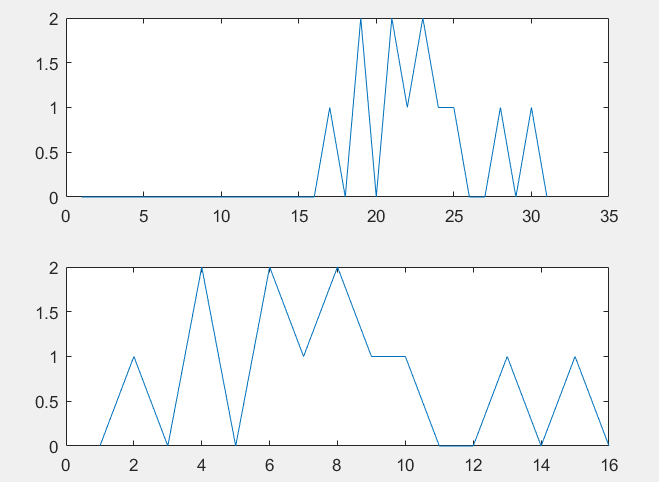
\includegraphics[width=0.6\linewidth]{Corr}}
\caption{Результаты корреляции.}
\end{figure}

Время осуществления корреляции:\\ 
Взаимной: 0.0011\\
Быстрой: 3.5244e-04\\

Как мы видим из времени вычисления, подсчеты с помощью быстрой корреляции производятся быстрее.
\newpage
\paragraph{5. Выводы\\\\}
Цифровая обработка, в отличие от аналоговой, традиционно используемой во многих радиотехнических устройствах, является более дешевым способом достижения результата, обеспечивает более высокую точность, миниатюрность и технологичность устройства, температурную стабильность.

При обработке цифровых сигналов радиолокатора используются алгоритмы цифровой фильтрации и спектрального анализа (вычисление дискретного и быстрого преобразования Фурье — ДПФ и БПФ), алгоритмы корреляционного анализа, обратной свертки, специальные алгоритмы линейного предсказания.

В системах обработки звука цифровые процессоры обработки сигнала решают задачи анализа, распознавания и синтеза речи, сжатия речи в системах телекоммуникации. Для систем обработки изображений типовыми задачами являются улучшение изображений, сжатие информации для передачи и хранения, распознавание образов. При обработке цифровых звуковых сигналов используются алгоритмы цифровой фильтрации и спектрального анализа (вычисление ДПФ и БПФ), алгоритмы корреляционного анализа, обратной свертки, специальные алгоритмы линейного предсказания.

\end{document}